\chapter{Preliminaries\label{chap:preliminaries}}

% Signposting
In this chapter, an overview of subjects that this work builds on is given.
The first section discusses propositional satisfiability, as this is the declarative paradigm the presented algorithm builds on.
In the second and last section, bi-objective optimization is described, starting from a general perspective and ending up with notation used for bi-objective optimization in the context of propositional logic.

\section{Propositional Satisfiability\label{sec:sat}}

% Propositional logic and SAT
For a Boolean variable $x$ there are two literals, the positive $x$ and the negative $\lnot x$. 
A clause $C$ is a set of (disjunction over) literals and a CNF formula $\formula$ is a set of (conjunction over) clauses.
A truth assignment $\sol$ maps boolean variables to $1$ (true) or $0$ (false).
The semantics of truth assignments are extended to a clause $C$ and a formula $\formula$ in the standard way: $\sol(C) = \max\{ \sol(l) \mid l \in C\}$ and $\sol(\formula) = \min\{\sol(C) \mid C \in \formula\}$.
When convenient, we view assignments $\sol$ over a set $X$ of variables as sets of literals $\sol = \{ x \mid x \in X,  \sol(x) = 1\} \cup \{ \lnot x \mid x \in X, \sol(x) = 0\}$.
An assignment $\sol$ for which $\sol(\formula) = 1$ is a solution to $\formula$.
The set of variables and literals appearing in $\formula$ are $\var(\formula)$ and $\lit(\formula)$, respectively.  
The propositional satisfiability (SAT) problem asks whether for a given formula $\formula$, a solution exists.
A formula $\formula$ is satisfiable if it has solutions, otherwise it is unsatisfiable.

% Example: SAT
\begin{example}
  Take the propositional formula $\formula_1 = a \land \lnot b$ over variables $\var(\formula_1) = \{a,b\}$.
  It is satisfiable since the assignment $\sol=(a,\lnot b)$ has $\sol(\formula_1)=1$.
  The formula $\formula_2 = a \land \lnot a$ on the other hand is not satisfiable since no assignment $\sol$ with $\sol(\formula_2)=1$ exists.
\end{example}

% SAT solvers
A SAT solver is an algorithm that determines the satisfiability of a given formula $\formula$.
If the formula is satisfiable, it returns ``satisfiable'' (SAT) and a solution $\sol$ with $\sol(\formula)=1$;
if it is unsatisfiable, it returns ``unsatisfiable'' (UNSAT).

% SAT as a declarative modelling language
The SAT problem was proved $\mathcal{NP}$-complete in~\textcite{DBLP:conf/stoc/Cook71}.
This result is very central to its modern day use as a declarative programming approach to solving other $\mathcal{NP}$-complete problems by encoding them as a propositional formula first, solving them with a SAT solver and then decoding the solution to the original problem context.
The advantage of using SAT as a declarative programming language for solving other problems comes from the fact that---even though SAT is $\mathcal{NP}$-complete, and it is unclear if a polynomial time algorithm for solving it exists---conflict-driven clause learning solvers~\autocite{handbook2-cdcl} for SAT are efficient in practice and can solve problems with hundred-thousands of variables and clauses\TODO{ check claim}.

% Example: SAT modelling
\begin{example}
  Consider the problem of whether to wear tie and shirt to a given event with the following constraints:
  (i)~one should not wear a tie without a shirt, (ii)~not wearing a tie nor a shirt is impolite, and (iii)~wearing a shirt and a tie is considered overdressed.
  To solve this problem with the help of SAT, it can be encoded to propositional logic by introducing variables $v_\text{shirt}$ and $v_\text{tie}$ that represent if a shirt or a tie is worn.
  The constraint can then be encoded as the following clauses:
  $\clause_\text{(i)} = \lnot v_\text{tie} \lor v_\text{shirt}$, $\clause_\text{(ii)} = v_\text{tie} \lor v_\text{shirt}$ and $\clause_\text{(iii)} = \lnot v_\text{tie} \lor \lnot v_\text{shirt}$.
  The formula $\clause_\text{(i)} \land \clause_\text{(ii)} \land \clause_\text{(iii)}$ can then be solved with a SAT solver, which will return the satisfying assignment $\{ v_\text{shirt}, \lnot v_\text{tie} \}$.
  This solution is decoded as it being appropriate to wear a shirt but no tie.
  \TODO{can I use this example?}
\end{example}

In this work, w.l.o.g.\ we assume that all formulas are satisfiable\TODO{ relevant?}.

\subsection{Incremental SAT Solving under Assumptions\label{sec:inc-sat}}

% Incremental SAT solving
It is common that algorithms that solve problems with the help of SAT solvers produce a series of SAT problems that only differ slightly.
To be able to solve these sub-problems more efficiently, most modern SAT solvers provide an incremental interface that allows for retaining information learned in previous solver calls~\autocite{DBLP:journals/entcs/EenS03,handbook2-cdcl}\TODO{ check if new CDCL chapter can be referenced}.
In order for the learned information from previous solver queries to still hold for subsequent calls, it is only possible to add clauses to the solvers internal formula, not remove them.
In addition, incremental SAT solvers support solving under assumptions.
The assumptions $\assump$ are a set of literals that are treated as unit clauses, i.e., a solver call with internal formula $\formula$ and assumptions $\assump$ either returns SAT and a solution $\sol \supset \assump$, or UNSAT and a subset $\core \subset \{\lnot l \mid l\in\assump\}$ such that $\formula \land \bigwedge_{l \in \core} (\lnot l)$ is unsatisfiable.
The subset $\core$ is called an unsatisfiable \emph{core} and, intuitively, is an explanation for the unsatisfiability of the query.

\subsection{Maximum Satisfiability\label{sec:max-sat}}

% MaxSAT
Maximum satisfiability (MaxSAT) is the optimization variant of the decision SAT problem.
In it, the goal is to find a solution that satisfies as many of the given clauses as possible.
Most commonly and in this work, MaxSAT refers to the extension of weighted partial MaxSAT, in which a set of \emph{hard} clauses $\formula$ and another set of \emph{soft} clauses $\softs$ are given.
Each clause $\clause \in \softs$ is assigned a weight $w_\clause$ and a solution $\sol$ that satisfies $\formula$ while minimizing $\sum_{\clause\in\softs \mid \tau(\clause)=0} w_\clause$ is optimal for the problem.

% MaxSAT as a modelling language
In the same way that SAT can be used as a declarative language to solve other decision problems, MaxSAT can be used to solve other optimization problems.

\subsection{Encoding Cardinality Constraints\label{sec:card-const}}

% Cardinality constraints
A common type of constraint to appear when encoding problems into SAT is that of a cardinality constraint.
Cardinality constraints, informally speaking, enforce a bound on how many literals in a set can be assigned to true.
Formally, for a set $L$ of literals and a bound $k \in \mathbb{N}$, $\texttt{As-CNF}\left(\sum_{l \in L} l \circ k\right)$ denotes a CNF formula that encodes the linear inequality $\sum_{l \in L} l \circ k$, where $\circ \in \{ ,< ,> ,\geq, \leq, =\}$.
Numerous methods of forming such CNF formulas are known~\autocite{DBLP:conf/cp/BailleuxB03}.

% Totalizer encoding
In this work we make use of the totalizer encoding.
Given a set $L$ of $n$ input literals and a bound $k=1, \ldots, n$, the (incremental) totalizer~\autocite{DBLP:conf/cp/BailleuxB03,DBLP:conf/cp/MartinsJML14} encoding produces a CNF formula $\tot(L, k)$ that defines a set $\{\ov{L}{1}, \ldots, \ov{L}{k}\} \subset \var(\tot(L))$ of \emph{output literals} that---informally speaking---count the number of literals in $L$ assigned to true by solutions to $\tot(L)$:
if $\tau$ is an assignment that satisfies $\tot(L)$, then $\tau(\ov{L}{b}) = 1$ if $\sum_{l \in L} \tau(l) < b$\TODO{ point out that iff (or $\leftarrow$) are possible as well, but we only need upper bounds}.
The incremental totalizer supports both increasing the bound $k$ and adding new input literals without having to rebuild the whole formula:
we have that $\tot(L, k) \subset \tot(L, k')$ and $\tot(L, k) \subset  \tot(L \cup L', k)$ hold for any bound $k' > k$ and set $L'$ of literals for which $L \cap L' =  \emptyset$. 
We use $\ove{L}{k}$ as a shorthand for the literal $\ov{L}{k+1}$.
We note that the assignments of the auxiliary variables of the totalizer encoding are functionally defined by the assignment of the input and output variables.
As such we will leave them out from the solutions we describe in favour of brevity and clarity of examples. 

\section{Bi-Objective Optimization and Pareto Optimality\label{sec:biopt}}

% Multiobjective optimization
Multi-objective optimization is the problem of optimizing $\nobj$ objective functions with the decision variable $x$, while $x$ is from a feasible set $\feasible$~\autocite{Ehrgott2005-1}.
W.l.o.g., we assume that all optimizations seek to minimize the objective function.
Formally a multi-objective optimization problem (MOOP) is the following:
\begin{equation}\label{eq:moop}
  \min (\generalobj_1(x),\dots,\generalobj_\nobj(x))\ \text{s.t.}\ x\in \feasible.
\end{equation}

% Pareto optimality
For multi-objective optimization problems, since the objectives might be in conflict with each other, no single optimal solution exists.
However, the notions of domination and pareto optimality can be used to define what a minimal point for multiple objective functions is.
\begin{definition}[Domination~\autocite{Ehrgott2005-2}]
  Given a MOOP as defined in \cref{eq:moop} and two solutions $x,x' \in \feasible$, $x$ dominates $x'$ (w.r.t.\ $\generalobj_1,\dots,\generalobj_\nobj$) if (i)~$\generalobj_i(x) \leq \generalobj_i(x')$ for $i=1,\dots,\nobj$, and (ii)~$\generalobj_i(x) < \generalobj_i(x')$ for some $i\in\{1,\dots,\nobj\}$.
  We represent $x$ dominating $x'$ as $x \prec x'$.
\end{definition}
\begin{definition}[Pareto optimality~\autocite{Ehrgott2005-2}]
  Given a MOOP as defined in \cref{eq:moop}, a solution $x \in \feasible$ is pareto-optimal (w.r.t.\ $\generalobj_1,\dots,\generalobj_\nobj$) iff there is no $x' \in \feasible$ such that $x' \prec x$, i.e., $x$ is not dominated by any other solution.
\end{definition}
When the objectives are clear from context, we will simply say that a solution $x$ is pareto-optimal.
Note that there can be multiple pareto-optimal solutions to a MOOP.
The set of all pareto-optimal solutions is called the pareto front (w.r.t.\ $\generalobj_1,\dots,\generalobj_\nobj$);
the tuple $(\generalobj_1(x),\dots,\generalobj_\nobj(x))$ for a pareto-optimal $x$---i.e., the image of $x$ in objective space---is a pareto point (which multiple solutions can correspond to).

% Bi-objective optimization in a SAT context
The subset of all multi-objective optimization problems which this work provides a solving algorithm for, is \emph{bi}-objective optimization, where the number of objective functions $\nobj=2$.
Furthermore, we restrict the objective functions to be linear.
Bi-objective optimization problems can be solved by many approaches (see \cref{chap:approaches} for more details), but in this work we focus on SAT-based approaches.
We therefore formalize the problem in a context of propositional satisfiability.
An objective $\Obj$ is a multiset of literals, which allows for representing objective functions with non-unit coefficients.
The value $\Obj(\sol)$ of a truth assignment $\sol$ under $\Obj$ is $\Obj(\sol) = \sum_{l \in \Obj} \sol(l)$, i.e., the number of the literals in $\Obj$ that $\sol$ assigns to $1$. 
Weighted objectives are represented by adding a literal multiple times.
Formalizing the objectives this way and encoding the feasible set $\feasible$ as a propositional formula $\formula$ is similar to MaxSAT, where $\formula$ resembles the hard clauses while the two objectives resemble two sets of (unit) soft clauses.
With our algorithm, we consider the task of computing a representative solution for each pareto point as well as the task of enumerating all solutions in the pareto front.

% Example: A bi-objective problem
\begin{figure}
  \begin{minipage}{0.36\textwidth}
    \footnotesize
    \begin{align*}
      \formula = &\{ \texttt{As-CNF}\left(\sum_ {x \in \Obj_\inc \cup \Obj_\dec} x \geq 3 \right), \\
        &(i_1 \lor i_2),  (i_2 \lor i_3), \\
        &(d_1 \lor d_2), (d_2 \lor d_3) \} \\ \\
      \Obj_\dec =&\{ d_1,d_2, d_3\}   \\ 
      \Obj_\inc =&\{ i_1,i_2, i_3\}  
    \end{align*}
  \end{minipage}
  \;
  \begin{minipage}{0.6\textwidth}
    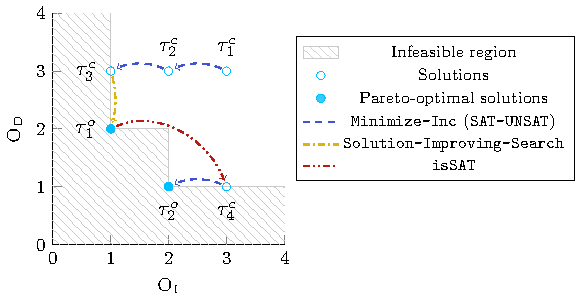
\includegraphics{search-trace.pdf}
  \end{minipage}
  \caption{Left: An example formula $\formula$ and two objectives $\Obj_\inc$ and $\Obj_\dec$.
    Right: the solution space of $\formula$ w.r.t.\ $\Obj_\inc$ and $\Obj_\dec$.
    The solutions $\tau^o_1$ and $\tau^o_2$ (solid points) are pareto-optimal, while $\tau^c_i$ for $i=1,\ldots,4$ are not.\label{fig:search-trace}}
\end{figure}
\begin{example}\label{ex:main}
  An example formula $\formula$ and two objectives $\Obj_\inc$ and $\Obj_\dec$ are shown on the left side of \cref{fig:search-trace}. 
  The solution space is illustrated on the right.
  The two solid dots correspond to the two pareto points of $\formula$ w.r.t.\ $\Obj_\inc$ and $\Obj_\dec$. 
  Examples of pareto-optimal solutions corresponding to these points are $\sol^o_1 = \{d_1, d_3, i_2, \lnot d_2, \lnot i_1, \lnot i_3\}$ and $\sol^o_2 = \{i_1, i_3, d_2, \lnot i_2, \lnot d_1, \lnot d_3\}$.
  The solution $\sol^c_3 = \{d_1, d_2, d_3, i_2, \lnot i_1, \lnot i_3\}$ is dominated by $\sol^o_1$ ($\sol^o_1 \prec \sol^c_e$) because $\Obj_\inc(\sol^o_1) \leq \Obj_\inc(\sol^c_3)$ and $\Obj_\dec(\sol^o_1) < \Obj_\dec(\sol^c_3)$.
\end{example}

% Proposition: Ordered pareto front
An important property of pareto-optimal solutions to bi-objective problems is summarized by the next proposition.
\begin{proposition}[Adapted from~\autocite{DBLP:conf/aaai/HartertS14}] \label{prop:biobjective}
  Sorting the pareto-optimal solutions of $\formula$ w.r.t.\ increasing values of $\generalobj_1$ is equivalent to sorting them w.r.t.\ decreasing values of $\generalobj_2$ and vice-versa.
\end{proposition}

% Example: Orderd pareto front
\begin{example}
  Consider the formula $\formula$, the objectives $\Obj_\inc$ and $\Obj_\dec$ and the two pareto-optimal solutions $\sol^o_1$ and $\sol^o_2$ from \cref{fig:search-trace} and \cref{ex:main}.
  By the definition of pareto-optimality, lowering the value of one objective of a pareto-optimal solution has to increase the value of the other;
  we have $\Obj_\inc(\sol^o_1) = 1 < 2 = \Obj_\inc(\sol^o_2)$ and $\Obj_\dec(\sol^o_1) = 2 > 1 = \Obj_\dec(\sol^o_2)$.
\end{example}